\documentclass[11pt]{article}
\usepackage[margin=1in]{geometry}
\usepackage{amsmath,amssymb,graphicx,booktabs,xcolor,hyperref,caption}
\usepackage[numbers,sort&compress]{natbib}
\hypersetup{colorlinks,linkcolor=blue!50!black,citecolor=blue!50!black,urlcolor=blue!50!black}
\newcommand{\todo}[1]{\textcolor{red}{[TODO: #1]}}
\newcommand{\vone}[1]{\textcolor{blue!60!black}{[[v1: #1]]}}
\newcommand{\E}{\mathbb{E}}
\graphicspath{{figs/}}
\title{Digital twins that forecast operation best learn the controller's co-movement, not the system's response}
\newcommand{\pancreasarx}{Supplementary Note~7}
\newcommand{\pancreasarxnumbers}{reactive loop, ARX(6/12/24) per-patient median learned/true 6.8/2.1/2.5 over 23 patients, with 10/5/7 of 68 cells excluded for divergent free simulation; meal-bolused loop $-0.01$/$-0.03$/$-0.05$, positive in 16/13/15 of 23 patients, no exclusions; linear twin 0.42 and 0.10 on the same logs; on designed open-loop logs ARX(6/12/24) 0.20/0.56/0.90 and the linear twin 1.00, 25 patients, no divergence}
\author{Debojit Biswas\\[2pt]\small Florida Atlantic University, Boca Raton, FL, USA\\\small \texttt{dbiswas2015@fau.edu}}
\date{}
\begin{document}
\maketitle

\begin{abstract}
Digital twins of controlled systems are trained on operational logs and asked what if the inputs changed. On a synthetic plant, a diabetes simulator and a building emulator over three heating periods, we show that the devices which make neural simulators roll out well on operational data---simulation-error training and input-noise injection---teach them the co-movement the controller induces rather than the system's response. Trained on operational logs, simulation-error twins recover 0.3--0.8 of the true heating effect at 6~h and 0.14--0.29 at 24~h while predicting ordinary operation best; replaying the same input open-loop with its days permuted within weather strata, which removes only its alignment with the unlogged disturbance, restores the effect (0.74--0.99). The bias is invisible to hold-out validation, ensembles and conformal intervals; plans through such twins track an out-of-range set-point change worse than the building's own controller, and twin-derived insulin doses cause severe hypoglycaemia in half to two-thirds of the virtual patients. The classical direct method on the same logs gives 0.9--1.7 of the truth but fails where the controller acts on information the log lacks. A logged $\pm2$-K set-point dither, costing 0.9--1.0~K of comfort and 15--28\% of heating energy, restores 0.45--1.1 of the effect.
\end{abstract}

\section*{Introduction}
A digital twin is a model that will be trusted to answer questions its training data never asked. The data are operational: a building logged under its thermostat, an insulin pump under its control algorithm, a plant under its regulator. The questions are interventional: what if the set-point schedule were changed, what if the heat pump were curtailed, what if the bolus were larger. The recipe that has become standard is to train a flexible sequence model---a recurrent network, a transformer, a neural differential equation, or a pretrained time-series foundation model fine-tuned on the log---to reproduce the log, to validate it on held-out operational data, and to use it for the interventional question, with an ensemble or a conformal interval to say how far it can be trusted.

Control theory settled the underlying question fifty years ago. Data collected under feedback can be uninformative about the plant, a model fitted by output error to such data converges to a mixture of the plant and the regulator inverse, and the remedies are known: a prediction-error model with a noise model, the indirect and two-stage methods when a reference signal is logged, and designed excitation at least cost \citep{gustavsson1977,ljung1999,forssell1999,vandenhof1993,bombois2006}. The building-identification community drew the practical conclusion a decade ago \citep{bacher2011,privara2013}. Neural system identification knows that simulation-error training is the output-error estimator of that theory; what the learned-simulator literature has not asked is what the output-error identity implies for a twin trained on closed-loop logs and used for a what-if.

This paper asks that question on three systems whose exact interventional answer is computable: a synthetic thermal plant, the UVA/Padova-class type-1 diabetes simulator with thirty virtual patients, and a community building emulator evaluated within its operating range over three heating-season periods, with replicated logs, five training seeds and bootstrap intervals, under a protocol fixed before the runs. We find that the modern recipe learns the co-movement that the controller induces: trained on operational logs, simulation-error twins recover 0.3--0.8 of the true heating effect at 6~h and 0.14--0.29 at 24~h, unchanged across a five-fold range of model size (and, in the synthetic plant, across a hundred-fold range of data volume), while being the best predictors of ordinary operation in the same data; a linear simulation-error twin of the diabetes simulator recovers 0.10--0.42 of the insulin effect. The classical direct method (ARX of order 12--48 and a state-space model), applied to the same logs, estimates the heating effect at 0.88--1.65 of the truth---over in one period, under in another---and fails where the controller anticipates what the log does not contain; with a logged set-point dither of $\pm2$~K the direct method estimates it at 0.76--1.12 (ARX(48) and state-space) and the simulation-error twins at 0.55--0.87. An open-loop replay of the operational input with its days permuted---within weather strata, so that its spectrum, its correlation with the logged weather and the temperature range are kept and only its alignment with the unlogged disturbance is removed---restores the effect for the simulation-error twins (0.74--0.99) and the clean transformer and most of it for the noise-injected families (the direct methods were never deprived of it), which locates the failure in the controller's co-movement rather than in the excitation. We show why the failure is invisible to hold-out error, ensembles and conformal intervals and not detected by pessimistic planning, what it costs at the level of decisions (building set-point changes tracked worse than by the building's own controller; severe hypoglycaemia in half to two-thirds of the virtual patients), and what did not help: a covariate-conditioned foundation model that did not, within our budget, learn the actuator effect even from designed data, a physically structured model with a free innovations gain, and instrumental corrections beyond the dither itself. The conclusion is uncomfortable but useful: for the question digital twins \citep{strachan2016twin} are built to answer, the field's default devices---simulation-error training and input-noise injection---replaced, rather than extended, a practice that already knew the failure, and the fix costs a few per cent of energy at its smallest useful amplitude.

\section*{Related work}
\paragraph{Closed-loop identification.} That data collected under feedback can be uninformative about the plant, and that a model fitted by output error on such data converges to a mixture of the plant and the regulator inverse weighted by the share of input power that came from external excitation, are results of the 1970s--1990s \citep{gustavsson1977,soderstrom1989,ljung1999,forssell1999}; the linear law in Methods is the output-error bias formula of \citet{forssell1999} written for learned simulators (for a causal, finite-memory model class the limit is the input-spectrum-weighted projection, of which the scalar excitation share is an approximation), and the remedies we test---a direct prediction-error model with a noise model, the indirect and two-stage methods with a logged reference \citep{vandenhof1993}, and designed excitation at least cost \citep{bombois2006,hjalmarsson2005}---are theirs. The building-identification literature drew the practical conclusion long ago \citep{bacher2011,privara2013}. Our contribution is not the law but the demonstration that the learned-simulator pipeline of the 2020s violates it in a way its own validation cannot see, the measurement of what that costs at the level of decisions, and the finding that the classical direct method, applied to the same operational logs, estimates the effect at 0.88--1.65 of the truth in the feedback-dominated building (over-estimating in one period, under-estimating in another)---and fails where the controller acts on information the log does not contain.

\paragraph{Policy-induced confounding in machine learning.} The same mechanism appears as causal confusion in imitation learning, where a learner copies the demonstrator's reaction to a variable it should ignore \citep{dehaan2019}, and its instrumental repair with lagged exogenous signals \citep{swamy2022}, like the perturbed executed actions of DART \citep{laskey2017dart}, is the analogue of our logged dither; \citet{ortega2021} describe the delusions of sequence models trained on interaction logs and act under them, which is the foundation-model version of our result. Confounded off-policy and model-based evaluation give bounds on what a world model fitted to confounded logs can say about a new policy \citep{tennenholtz2020,namkoong2020,brunssmith2021,shi2022}, and time-series treatment-effect estimators under hidden confounding \citep{bica2020,melnychuk2022} and proximal or instrumental estimators \citep{hartford2017,rothenhausler2021} are the causal-inference tools that a twin would need and that the standard pipeline does not use. Model-based offline reinforcement learning penalises ensemble disagreement to keep a planner where the model is trustworthy \citep{yu2020mopo,kidambi2020morel}; we test whether that pessimism detects controller-induced bias, which is not disagreement.

\paragraph{The recipes under test.} Two devices make neural simulators roll out well on operational data and are the subject of this paper. \emph{Simulation-error (multi-step) training}, in which the model is unrolled and its rollout is fitted to the log, is the recipe of neural system identification and continuous-time neural models \citep{forgione2021,beintema2021}; \emph{input-noise injection} during teacher-forced training, which stabilises rollouts by exposing the model to perturbed inputs, is the device of learned physical simulators \citep{sanchez2020gns,pfaff2021meshgraphnets}, and scheduled sampling, which feeds the model its own predictions instead \citep{bengio2015scheduled}, is its cousin. The one-step Gaussian ensembles of model-based reinforcement learning \citep{chua2018pets,janner2019mbpo,yu2020mopo} and the latent one-step models of world-model agents \citep{hafner2020dreamer} are teacher-forced next-step learners, closest to the clean next-step families here, whose behaviour we find recipe- and architecture-dependent.

\paragraph{Uncertainty under interventional shift.} Conformal prediction is valid under exchangeability \citep{vovk2005conformal}; weighted conformal methods handle covariate shift with a known density ratio \citep{tibshirani2019}, which is singular when a deterministic controller sets the input, and adaptive methods recover coverage only after the shift is observed \citep{gibbs2021}. Our conformal experiment is a test of what practitioners do, not of what the theory promises.

\section*{Results}
\paragraph{Setting and protocol.} Three systems have a computable interventional answer: a synthetic two-node thermal plant under PI control with a hidden heat disturbance; the UVA/Padova-class type-1 diabetes simulator with thirty virtual patients under a hybrid closed-loop insulin controller with unlogged meals; and the IBPSA BOPTEST residential heat-pump emulator under its embedded controller with unlogged occupancy, over three four-week heating-season periods. In the building every model is trained on an \emph{operational} log, on three \emph{dithered} logs (a logged random set-point offset of $\pm2$~K; same weather and occupancy) and on \emph{designed} logs (random actuator schedule), and is scored on (i) its response to a step in heat-pump modulation from seven operational start states 48~h apart, relative to the emulator's exact response (\emph{learned fraction}; the 24-h value is the pre-stated primary, reported at 3--48~h and for a smaller $+0.1$ step that stays closer to the operating range); (ii) its rollout error on the operational test weeks (\emph{operational error}, what practitioners validate on); (iii) its in-range rollout error on a designed schedule around the test weeks' operating level; and (iv) the coverage of split-conformal 90\% intervals calibrated on operation. Neural families use five seeds; intervals are hierarchical bootstraps over seeds and start states. A family enters the headline comparison if, trained on designed data, it recovers the step response within $\pm50\%$ with rollouts better than persistence (Supplementary Table~1). The protocol, its pre-stated predictions and every change made after seeing data are in Methods, Extended Data Tables~1--2 and Supplementary Note~12, which gives the full account of every result below.

\begin{table}[t]\centering\footnotesize
\caption{\textbf{Learned fraction of the true heating effect, BOPTEST heat-pump building, from operational start states.} Twins trained on the operational log (24-h fraction, mean over seeds with 95\% hierarchical bootstrap interval over seeds and the seven 48-h-spaced start states; 6-h fraction, mean and the same interval), on three $\pm2$-K dithered logs (24-h, range over logs) and on designed logs (24-h, mean), for three heating-season periods. True 24-h effects 2.55, 2.97 and 2.70~K (s.d.\ over starts 0.33, 0.37, 0.40); 6-h effects 0.92, 1.13, 0.96~K. Seeds in parentheses; for the single-fit linear models the interval is a bootstrap over the seven starts only. The interval statistic is the ratio of the mean learned to the mean true effect over resampled seeds and starts; the point estimate is the mean of per-seed ratios. The grey-box model with a free innovations gain fails the designed-data capability criterion and is shown for completeness; the 48-unit clean next-step GRU is shown although its rollouts are worse than persistence. Supplementary Table~6 gives every horizon and the $+0.1$ step.}\label{tab:v1}
\resizebox{\textwidth}{!}{\begin{tabular}{lccc|ccc|ccc|ccc}\toprule
 & \multicolumn{3}{c|}{operational log, 24 h} & \multicolumn{3}{c|}{operational log, 6 h} & \multicolumn{3}{c|}{operational + $\pm2$-K dither (3 logs)} & \multicolumn{3}{c}{designed data}\\
family & P1 & P2 & P3 & P1 & P2 & P3 & P1 & P2 & P3 & P1 & P2 & P3\\\midrule
GRU, simulation-error (5 seeds) & 0.22 [0.16, 0.30] & 0.14 [0.08, 0.20] & 0.28 [0.20, 0.41] & 0.59 [0.44, 0.79] & 0.32 [0.24, 0.39] & 0.75 [0.47, 1.12] & 0.67--0.74 & 0.55--0.63 & 0.67--0.87 & 1.04 & 1.06 & 1.27\\
GRU 256 units, simulation-error (3, 2, 2) & 0.19 [0.16, 0.24] & 0.21 [0.16, 0.26] & 0.29 [0.25, 0.33] & 0.56 [0.41, 0.74] & 0.48 [0.36, 0.59] & 0.79 [0.52, 1.15] & 0.72 (one log) & -- & -- & 0.86 & 1.03 & 1.27\\
GRU, next-step + noise (5) & 0.13 [0.06, 0.23] & 0.06 [0.02, 0.13] & 0.19 [0.10, 0.30] & 0.32 [0.21, 0.46] & 0.18 [0.06, 0.33] & 0.64 [0.32, 1.08] & 0.44--0.48 & 0.22--0.26 & 0.44--0.58 & 1.28 & 0.66 & 0.93\\
Transformer, next-step + noise (5) & 0.36 [0.22, 0.50] & 0.15 [0.08, 0.21] & 0.22 [0.12, 0.30] & 0.45 [0.23, 0.70] & 0.22 [0.09, 0.35] & 0.51 [0.28, 0.76] & 0.60--0.70 & 0.44--0.66 & 0.60--0.70 & 0.90 & 0.50 & 0.80\\
Transformer, next-step (5) & 0.78 [0.65, 0.94] & 0.63 [0.44, 0.87] & 0.48 [0.40, 0.61] & 0.73 [0.59, 0.88] & 0.51 [0.35, 0.72] & 1.06 [0.73, 1.42] & 0.65--0.81 & 0.45--0.77 & 0.53--0.65 & 0.98 & 1.02 & 0.75\\
Transformer 4 layers, next-step (2) & 0.72 [0.58, 0.92] & 0.63 [0.47, 0.83] & 0.48 [0.23, 0.74] & 0.75 [0.59, 0.88] & 0.47 [0.36, 0.58] & 1.13 [0.69, 1.64] & -- & -- & -- & 0.75 & 1.01 & 0.65\\
GRU, next-step (5; unstable) & 2.17 [1.01, 3.48] & 2.75 [1.90, 3.71] & 2.39 [0.95, 3.82] & 0.70 [0.31, 1.17] & 1.04 [0.65, 1.42] & 1.38 [1.07, 1.70] & 1.44--1.72 & 1.74--2.16 & 0.49--0.96 & 1.09 & 1.14 & 0.79\\
ARX(2) & 1.16 [1.07, 1.28] & 1.44 [1.31, 1.58] & 0.98 [0.87, 1.09] & 1.21 [1.07, 1.42] & 1.18 [1.11, 1.26] & 1.11 [1.00, 1.25] & 0.73--0.85 & 0.75--0.84 & 0.75--0.82 & 1.33 & 1.39 & 1.43\\
ARX(12) & 1.55 [1.43, 1.74] & 1.14 [1.04, 1.25] & 0.90 [0.81, 1.00] & 1.37 [1.21, 1.58] & 1.15 [1.08, 1.22] & 1.17 [1.05, 1.32] & 0.69--0.82 & 0.69--0.75 & 0.72--0.77 & 1.09 & 1.20 & 1.15\\
ARX(24) & 1.62 [1.49, 1.79] & 1.12 [1.03, 1.24] & 0.94 [0.85, 1.05] & 1.37 [1.22, 1.57] & 1.14 [1.07, 1.21] & 1.14 [1.02, 1.30] & 0.73--0.81 & 0.66--0.75 & 0.72--0.79 & 1.08 & 1.18 & 1.12\\
ARX(48) & 1.40 [1.29, 1.56] & 1.11 [1.01, 1.22] & 0.88 [0.79, 0.99] & 1.28 [1.14, 1.48] & 1.10 [1.04, 1.18] & 1.11 [0.99, 1.26] & 0.83--0.87 & 0.82--0.83 & 0.76--0.86 & 1.04 & 1.10 & 1.07\\
PEM state-space (2) & 1.64 [1.50, 1.82] & 1.65 [1.51, 1.80] & 1.21 [1.08, 1.35] & 1.35 [1.20, 1.56] & 1.26 [1.19, 1.34] & 1.22 [1.08, 1.36] & 1.01--1.12 & 0.94--1.05 & 0.94--1.06 & 1.38 & 1.47 & 1.45\\
grey-box 2R2C, free gain & 0.29 [0.27, 0.32] & 0.51 [0.47, 0.56] & 0.23 [0.20, 0.25] & 0.44 [0.39, 0.51] & 0.49 [0.46, 0.52] & 0.43 [0.38, 0.48] & 0.09--0.24 & 0.09--0.17 & 0.13--0.24 & 0.49 & 0.08 & 0.21\\
\bottomrule\end{tabular}}\end{table}

\paragraph{Both estimators are biased by the operational regime; the simulation-error recipe by far the most.} Table~1 and Fig.~1 give the learned fraction by family, training regime and period. A GRU trained by simulation error on the operational log learns $0.22$ [95\% CI 0.16--0.30], $0.14$ [0.08--0.20] and $0.28$ [0.20--0.41] of the true 24-h heating effect in the three periods; a 256-unit GRU learns 0.19--0.29; a next-step GRU or transformer trained with the input-noise injection that stabilises rollouts learns 0.06--0.36. These are the twins with the lowest error on the operational test weeks in every period (0.11--0.49~K), which is why operational validation selects them. The shortfall grows with horizon: the same twins learn 0.59 [0.44--0.79], 0.32 [0.24--0.39] and 0.75 [0.47--1.12] of the effect at 6~h, where every arm of the query is inside the training range, and 0.14, 0.10 and 0.19 at 48~h---in two of three periods they reproduce most of the fast air response, in all three they lose the slow accumulation that the controller cancels---and it is not an artefact of the step leaving the operating range, since a $+0.1$ step from the same states gives the same fractions (0.26, 0.15 and 0.36 at 24~h; Supplementary Tables~6--7). The same architectures trained on designed data recover the 24-h effect to 0.50--1.28. The classical direct method on the same logs estimates the effect at 0.88--1.65 of the truth, in a direction that depends on the period: ARX models of order 12--48 learn 1.40--1.55, 1.11--1.14 and 0.88--0.90, and a second-order innovations-form state-space model 1.64, 1.65 and 1.21, of which about 1.4 is structural (it over-estimates on designed data too), with operational errors of 0.30--1.31~K. Within one architecture the training device decides (Fig.~2): the clean next-step transformer keeps $0.78$ [0.65--0.94], $0.63$ [0.44--0.87] and $0.48$ [0.40--0.61] of the effect, robustly across a sixteen-run recipe sweep, and pays for it in operational error (0.29--0.66~K); the same transformer with noise injection learns 0.36, 0.15 and 0.22; the clean next-step GRU is unstable at 48 units and, at 256 units, where it reaches the simulation-error GRU's operational accuracy, learns its fraction too (0.25). Whatever buys operational accuracy---the simulation-error loss, input-noise injection or capacity---buys the co-movement. A sign-constrained grey-box model fitted by simulation error puts the slab capacitance two orders of magnitude above its designed-data value: the slow mode the controller cancels is unidentifiable from operation, the classical informativity diagnosis in physical units. In the synthetic plant under pure feedback a 20th-order ARX reaches a relative error of 0.17 on a log from which simulation-error GRUs reach 1.03--1.27 and clean next-step GRUs and transformers 0.96--1.0, unchanged between $2{\cdot}10^3$ and $2{\cdot}10^5$ samples and between 8 and 256 hidden units; with an anticipating controller the ARX fails too, as the theory predicts.

\paragraph{What the simulation-error twin learns, and why the validation stack does not see it.} A simulator trained by simulation error converges to $\E[y\mid u,y_{\mathrm{hist}},x]=\mathcal G[u]+\E[v\mid u,y_{\mathrm{hist}},x]$, the true response plus the disturbance the controller reveals through the input (Methods, equation~(1)); under pure feedback its linear limit is the negative inverse controller. On the building the controller is known: fitted from the operational log ($R^2>0.99$), its inverse responds to the $+0.3$ step with $-0.19$, $-0.85$ and $-0.59$~K at 24~h, the truth with $+2.55$, $+2.97$ and $+2.70$~K, and the simulation-error GRU with $+0.56$, $+0.43$ and $+0.76$~K, a quarter to two-fifths of the way from the inverse to the plant. No twin reproduces the controller's inverse; every learned response is positive and a shrinking fraction of the truth with horizon (Extended Data Fig.~1). The scalar linear law gives the order of magnitude of the 24-h fraction on the dithered logs but predicts it across logs no better than their mean does, and says nothing about the horizon profile (Supplementary Table~5); the profile is the general identity's signature of a missing slow mode---the controller cancels slow excursions, so in the log a sustained rise in modulation is accompanied by a cold disturbance rather than a rising temperature. The test that separates this co-movement from the input's excitation is an open-loop \emph{replay}: the operational modulation sequence, cut into its 28 days and permuted, is applied open-loop in the emulator over the same weeks, keeping the weather, the occupancy schedule, the values and the within-day profile of the input and removing its alignment with the disturbance the controller was reacting to. Twins trained on such logs recover the effect: the simulation-error GRU 0.73--1.21 against 0.14--0.28, the noise-injected families 0.54--1.07 against 0.06--0.36, the clean transformer 0.96--1.60 (Supplementary Table~8). Because a whole-day permutation also removes the input's correlation with the logged weather and widens the temperature range, a \emph{weather-stratified} replay permutes days only within quartiles of the daily mean outdoor temperature, which keeps that correlation ($-0.34$ to $-0.62$ against $-0.52$ to $-0.70$) and a nearly operational range (17--25 against 20--24~$^\circ$C), and still restores the effect: the simulation-error GRU learns 0.74--0.99 at 24~h and 0.81--1.16 at 6~h, the clean transformer 0.84--1.27, the noise-injected transformer 0.42--0.80 and the noise-injected GRU 0.13--0.68 (Supplementary Table~9). The direct methods, which the operational log never deprived of the effect, move to their open-loop estimates. What the operational log withholds is therefore neither excitation nor independence from the logged weather but the independence of the input from the unlogged disturbance---the controller's co-movement. Three consequences follow. The error is a bias of the population optimum, flat in data and capacity. It is invisible to operational validation: the twins with the lowest operational error have the lowest learned fraction, and in the synthetic plant the error exceeds the ensemble spread 7--80-fold. And predictive intervals calibrated on operation do not transfer: on in-range interventional samples, 90\% conformal intervals of the simulation-error GRU cover 48, 81 and 40\% (transformer 80, 98 and 56\%; ARX(48) 90, 98 and 64\%) against 85--98\% on operation (Supplementary Table~3).

\paragraph{Decisions.} In the synthetic plant, input schedules optimised through operational-data simulation twins to reach a 3-K target are worse than doing nothing in 29 of 36 regime--seed cells and worse than the designed-data twins' plans in all, while the twins believe their plans succeed. In the building, with receding-horizon re-planning every 2~h through bootstrap ensembles of five twins (Fig.~4a), schedules from the operational twin track a set-point change inside the operating range to $0.66\pm0.28$~K (s.d.\ over five starts) against 0.47 for the building's own controller and 0.59 for a designed-data twin under the same planner, and a change that leaves the range to $1.41\pm0.46$~K against 0.53 and 0.58; a pessimistic penalty on ensemble disagreement \citep{yu2020mopo} reduces the out-of-range damage in 4 of 5 starts (to 0.72~K; paired improvement 0.68~K, s.d.\ 0.80, $p=0.13$) by keeping the plan in the controller's own territory, and degrades the dithered twin (0.32 to 0.57~K), which is the best controller we built. In the diabetes simulator, a correction-bolus calculator derived from each twin and applied to the true patient at a steady hyperglycaemia (Fig.~4b) gives, from the true effect, 2.8~U and no hypoglycaemia in 25 patients; from twins of the reactive pump loop, 6.9~U and glucose below 54~mg/dL in 12 of 23; from twins of the meal-bolused loop, no dose at all in 6 of 22 and severe hypoglycaemia in 15 of 22 (both $p<0.001$ against the reference).

\paragraph{What helps, and where the direct method stops.} A logged set-point dither of $\pm2$~K, which costs 0.9--1.0~K rms of zone temperature and 15--28\% of summed heat-pump modulation over the training month, moves the 24-h learned fraction to 0.55--0.87 for the simulation-error GRU (0.94--1.17 at 6~h), 0.45--0.81 for the clean transformer, 0.22--0.70 for the noise-injected families and 0.76--1.12 for ARX(48) and the state-space model, in every period and every dithered log (Fig.~3); the dose--response is monotone, $\pm0.5$~K costing 0.3~K and 4\% for a fraction of 0.51 (Supplementary Table~4). In the diabetes simulator the same device with a two-stage instrumental estimator \citep{angrist2009} reduces the overdoses (3 of 23 severe in either loop); beyond the dither, instrumental corrections add little. The direct method itself has a boundary: on the pump logs of the diabetes simulator, where the patient is nonlinear and meals are unlogged, ARX models of order 6--24 over-estimate the 4-h insulin effect 2.1--6.8-fold in the reactive loop (per-patient medians, 23 patients; a lower bound, since divergent free simulations are excluded), although on open-loop logs of the same patients ARX(24) recovers 0.90, and in the meal-bolused loop, where the controller acts on meals the log does not contain, estimate it as nothing ($-0.05$ to $-0.01$ of the truth, positive in 13--16 of 23 patients), as the theory of the direct method under anticipating control predicts. The linear simulation-error twin on the same logs learns 0.42 and 0.10 of the effect, with a positive 2-h effect---``insulin raises glucose''---in every meal-bolused cell (Supplementary Note~7).

\paragraph{What did not help.} Chronos-2 \citep{chronos2}, a covariate-aware time-series foundation model given the actuator and the weather as known future covariates, forecasts operation to 0.15~K after fine-tuning on the operational log but learns a 24-h heating response of 0.02~K; fine-tuned on designed data across six recipes it learns $-0.16$ to 0.44~K of a 2.4-K effect, fails the capability criterion, and its operational result is therefore not evidence about confounding (Supplementary Note~5).

\section*{Discussion}
Three things are established. A simulator trained by simulation error on operational data converges to the true response plus the disturbance the controller reveals through the input---an identity that is Pearl's \citep{pearl2009} and Forssell--Ljung's, restated---and every simulation-error and noise-injected family we tested behaves as the identity says: a positive response that is a shrunken plant response rather than the controller's inverse (the simulation-error GRUs 0.3--0.8 of the truth at 6~h and 0.14--0.29 at 24~h, the noise-injected families 0.06--0.36 at 24~h), decaying with horizon as the slow mode the controller cancels goes missing, not moving with data or capacity, and restored by an open-loop replay of the same input with its days permuted within weather strata, which keeps the input's spectrum, its weather correlation and the temperature range and removes only its alignment with the unlogged disturbance---the direct demonstration that the missing ingredient is the controller's co-movement, not excitation. Whatever buys operational rollout accuracy buys the co-movement; the clean next-step transformer is the one neural family that keeps about half or more of the 24-h effect, and pays for it in operational error. The failure is invisible to the validation stack because every element of that stack is evaluated under the operational law of the input; the twins that learn a fifth of the 24-h heating effect are the best predictors of operation, their ensembles disagree no more than well-trained twins, the simulation-error GRU's conformal intervals cover 40--81\% of in-range interventional outcomes at nominal 90\%, and a pessimistic planner improves their plans, where it does, by keeping them where the controller already went. The classical direct method, which the learned-simulator literature replaced rather than extended, estimates the effect at 0.88--1.65 of the truth on the same building data (0.76--1.12 once a dither is logged), and fails where the controller anticipates what the log does not contain.

What should a practitioner do? Log a small random perturbation of the set-point---$\pm0.5$~K costs 0.3~K of comfort and 4\% of heating energy over a month on this building and already restores half of the simulation-error twin's 24-h effect, $\pm2$~K costs 0.9--1.0~K and 15--28\% and restores 0.55--0.87---which buys most of the attainable accuracy for every working model family we tested except the noise-injected ones; before trusting a twin's what-if, compare its learned step response with that of a prediction-error model with a noise model fitted to the same log, and run the capability control---train the same model on designed data from the same system and check that it recovers a known effect---because two of the families we tested could not.

The limitations are plain. Every plant here is a simulator, which is what makes the exact interventional truth available; the one real dataset we examined elsewhere leaves the heater effect unidentified from its regulated weeks, consistent with the identity but not a quantitative test. The quantitative law is linear and scalar; on the building it gives the order of magnitude of the 24-h fraction on the dithered logs (within 0.1 in six of eleven, exceeded by 0.2--0.3 in period~3, and no better than the mean fraction across logs), is only an upper bound where the excitation is not exogenous, and does not describe the horizon profile, which is the signature of the missing slow mode; on the diabetes simulator we have ordinal agreement and replicated fractions. The direct method's period-dependent bias on the building is partly alignment too: on the shuffled-day replay ARX moves from 1.55 to 1.1--1.3 in period~1 and from 0.88 to 1.2--1.3 in period~3, 0.1--0.3 above its designed-data estimates, consistent with the within-day alignment the permutation preserves; we do not separate this further. The $+0.3$ step query, the pre-stated primary, leaves the training-log temperature range for most of its first day in two periods; a $+0.1$ step, whose intervention arm is in range 58, 57 and 81\% of its first day against 71, 79 and 80\% for the base arm, gives the same fraction, and we report every horizon for the headline families. The in-support test schedules could not be kept entirely inside the operational range without feedback, and we report in-range-only errors alongside. And the diabetes controller is a generic PID rather than a deployed algorithm. None of these changes the central comparison, which is between estimators on the same data.

\section*{Methods}
\paragraph{Synthetic plant.} A two-node thermal plant (air node $C_a=1$, mass node $C_m=30$, coupling $0.3$, losses $0.05$ and $0.02$, unit input gain; discretised exactly at unit step) is driven by a hidden AR(1) heat disturbance ($\rho=0.99$, s.d.\ $0.5$) on the air node and measured through a sensor with noise s.d.\ $0.02$ and quantisation $q\in\{0.01,0.5\}$. A PI controller ($k_p\in\{0.5,2,8\}$, $k_i=k_p/20$, anti-windup, input clipped to $[0,6]$) tracks a reference that equals the nominal set-point plus, in dithered regimes, random steps of amplitude $\sigma_r\in\{0,0.05,0.2,1\}$ held for 20--200 steps; an anticipation parameter $d\in\{0,0.8\}$ adds $-d\,q_t$ to the controller output (a controller that sees the disturbance). Logs of $N\in\{2{\cdot}10^3,2{\cdot}10^4,2{\cdot}10^5\}$ steps, three seeds. The query is the effect of a fixed designed binary sequence (600 steps, pulses 5--200 steps) relative to holding the operating input, from steady state; the score is the rms error of the predicted effect divided by the rms of the true effect. Designed logs for capability controls concatenate independent designed sequences. Linear estimators: ARX of order 2 and 20, a second-order output-error model fitted by simulation error, and two-stage least squares with the reference as instrument (432 cells, \texttt{c1\_synthetic.py}). Neural simulators: a GRU (32 hidden units) trained by simulation error over 150-step rollouts after a 50-step warm-up (1,500 Adam steps), ensembles of five; a GRU and a two-layer causal transformer (context 128) trained by next-step prediction with input-noise injection (6,000 steps; recipe validated on designed data, Supplementary Information). Planning: 300-step input schedules in $[0,6]$ optimised by gradient descent through the twin to track a $+3$-K target, applied open-loop to the noise-free plant. Capacity sweep: GRU hidden size 8--256, 3,000 steps, three seeds, closed loop $k_p=2$, $d=0.8$ versus designed data (\texttt{c10\_capacity.py}).

\paragraph{Theory.} Let $y=\mathcal G[u]+v$ with $\mathcal G$ the plant's causal response to the input path and $v$ the disturbance-driven part of the output, and let a simulator be trained by simulation error given a warm-up $y_{\mathrm{hist}}$ and logged drivers $x$. With a rich enough class the population minimiser is
\begin{equation}
\hat{\mathcal G}[u\mid y_{\mathrm{hist}},x]=\E[y\mid u,y_{\mathrm{hist}},x]=\mathcal G[u]+\E[v\mid u,y_{\mathrm{hist}},x],
\label{eq:identity}
\end{equation}
and under an intervention $\mathrm{do}(u=u^*)$ from the same warm-up the true output is $\mathcal G[u^*]+v$ with $\E[v\mid\mathrm{do}(u^*),y_{\mathrm{hist}},x]=\E[v\mid y_{\mathrm{hist}},x]$, so the twin's error is $\E[v\mid u^*,y_{\mathrm{hist}},x]-\E[v\mid y_{\mathrm{hist}},x]$: the part of the disturbance that the controller's production of $u^*$ reveals beyond what the warm-up already reveals. It is a property of the operational law, not of the sample size or the class. In the linear time-invariant case with plant $G$, disturbance model $H$, controller $u=C(r-y)+Fe$ and sensitivity $S=(1+GC)^{-1}$, the non-causal simulation-error limit is $\hat G=\gamma^2G+(1-\gamma^2)G_{\mathrm{op}}$ with $G_{\mathrm{op}}=(GF+H)/(F-CH)$ and $\gamma^2$ the coherence of $u$ with $r$ \citep{forssell1999,ljung1999}; under pure feedback $G_{\mathrm{op}}=-1/C$ \citep{gustavsson1977}, and causal parametric classes converge to the $\Phi_u$-weighted projection of this limit \citep{ljung1999}. One-step learners with history are the direct prediction-error method with a free noise model, consistent under feedback when the loop is informative and $F=0$ \citep{ljung1999,forssell1999}; with $F\neq0$ the regression of $y_{t+1}$ on $u_t$ given the past absorbs the part of $v$ that $u_t$ reveals (an omitted-variable bias), and in the synthetic plant the 20th-order ARX that is consistent at $F=0$ (relative error 0.17) has a relative error of about 1.0 at $F\neq0$ (anticipation 0.8) at every data volume. Planning: a planner that solves $\hat{\mathcal G}[u]=\Delta$ at steady state applies $u=\Delta/\hat g$, so the true change is $\Delta g/\hat g$; with integral action in the loop $G_{\mathrm{op}}(0)=0$ and $\hat g\to\gamma^2 g$.

\paragraph{Diabetes simulator.} \texttt{simglucose} 0.2.11 \citep{simglucose} (Dalla Man model \citep{dallaman2007}, UVA/Padova parameters), thirty virtual patients (adult, adolescent and child cohorts, ten each), 1-min integration, 5-min control and CGM (noise 5~mg/dL, 1-mg/dL resolution). Controller: insulin rate $=$ basal$\cdot(1+k_p e+k_i\sum e+k_d\Delta e)$ with $e=(\mathrm{CGM}-120)/100$, $k_p=1$, $k_i=0.01$, $k_d=2$, clipped to $[0,5\times$basal$]$, plus a meal bolus of a fraction $d\in\{0,0.7\}$ of CHO/CR at meal onset ($d=0$: fully reactive, unannounced meals); meals three per day at random times ($\pm1$~h) and sizes plus Poisson snacks, not logged; three meal-schedule seeds per patient and configuration; 14-day logs. Dither: additive basal offset $r\cdot$basal, $r\sim U(-0.5,0.5)$ held 30--120~min, logged. Capability control: a designed 14-day log (basal multiplied by $\{0,0.5,1,2\}$ held 30--180~min plus random boluses, meals unlogged); a patient enters the comparison if the twin trained on it recovers the 4-h effect of a 1-U bolus to a relative error below 0.5 (25 of 30 pass; median 0.14; the five failing patients are listed in Supplementary Information). Cells with $\ge50\%$ time below 70~mg/dL are excluded (a threshold set after a first version of the study). Query: blood-glucose difference with and without a 1-U bolus from the fasting steady state over 6~h. Twins: the linear simulation-error twin (exponential filter bank on insulin, ridge $10^{-4}$) and its two-stage version with the dither as instrument; a direct-method ARX comparator (orders 6--24; least squares on glucose and delivered insulin at 5-min steps, free simulation of a 1-U bolus from the fasting steady state) on logs regenerated under the same protocol with a stable seed, the linear twin refitted on the same regenerated logs (the first version of this comparator used the ten-adult logs of the first study version); ARX free simulations that diverge (non-finite or beyond $10^3$~mg/dL) are excluded and counted; the three meal seeds of a patient are near-replicates (meal-bolused loop: within-patient s.d.\ of the ARX(12) ratio 0.01 against 0.17 between patients; in the reactive loop the within-patient spread is dominated by the divergent cells), so statistics are per-patient medians over 23 patients per loop; neural twins in Supplementary Information. Dosing scenario: a constant carbohydrate drip tuned by slow integral control over 8~h to hold glucose near 180~mg/dL at basal insulin, then held constant; the reference effect of 1~U is computed at that operating point (so the reference calculator is exact by construction); each twin's calculator doses $60/|\text{effect}_{4\,\mathrm h}|$~U (cap 10~U; no dose if the effect is non-negative; meal seed 0), applied to the true patient; outcomes are glucose at 4~h, the minimum over 8~h and thresholds 70 and 54~mg/dL; one-sided Fisher's exact tests against the reference. The achieved steady state varied from 169 to 586~mg/dL across patients (the drip tuning does not converge for the most insulin-resistant), which is reported with the results.

\paragraph{Building emulator.} IBPSA Project~1 BOPTEST \citep{blum2021boptest} (commit 0f8a467), test case \texttt{bestest\_hydronic\_heat\_pump}, co-simulated through its FMU with \texttt{fmpy} at 15-min steps (the embedded controller runs inside the FMU; overrides through the test case's \texttt{ove*} inputs). Logged: zone temperature, applied heat-pump modulation, outdoor dry-bulb temperature, global horizontal irradiance, and the set-point tracked by the embedded controller. Not logged: occupancy and internal gains, slab and wall temperatures. Three periods, each a four-week training window followed by a two-week test window (days 7--35/42--56, 45--73/80--94, 300--328/335--349 of the weather year). Training logs per period: one operational log; three dithered logs (set-point $=$ schedule $+$ random offset $U(-2,2)$~K held 1--6~h; also $\pm0.5$ and $\pm1$~K in period~1); two designed logs (modulation held at random levels around the operating region for 1--12~h). Test material per period: an operational log of the test weeks; an in-range designed schedule (levels $\{1/3,2/3,1,4/3\}$ of the test weeks' mean operational modulation, held 15~min--1.5~h; 86, 69 and 49\% of samples inside the training log's temperature range); an out-of-range designed schedule (reported in Supplementary Information); and the step query from operational start states---seven start times exactly 48~h apart in the test weeks, the emulator replayed under embedded control to each and then run for 48~h with the modulation held at 0.4 and at 0.7, the difference being the exact effect (24-h effect 2.55, 2.97 and 2.70~K, s.d.\ 0.33, 0.37 and 0.40 across starts; an earlier version of this query had closer-spaced starts and an override fault, see Extended Data Table~2). Twins compute the same difference from the same 24-h warm-up and weather. Models: ARX of orders 2--48 (least squares); innovations-form state-space models of order 2--4 fitted by prediction error from six random initialisations; a sign-constrained 2R2C grey-box model with free innovations gain, likewise; GRU (48 units) by simulation error over 144-step rollouts after a 48-step warm-up (2,000 Adam steps); next-step GRU and two-layer causal transformer (48-dim, context 96) by teacher forcing (6,000 steps) with and without input-noise injection ($\sigma=0.1$ in normalised units); 256-unit GRUs and a 128-dim four-layer transformer on the GPU (Supplementary Information); five seeds for neural families (two to three for the GPU models). Recipe sweep (period~1, clean next-step families): hidden size $\{48,96\}$, learning rate $\{10^{-3},3\cdot10^{-3}\}$, steps $\{6000,10000\}$, two seeds, each recipe trained on a designed and on the operational log, the recipe with the lowest in-range designed-test error of its designed-data twin selected before its operational-data fraction was read (Supplementary Table~2). Evaluation: predictor through the warm-up, pure simulation thereafter; windows of 24~h warm-up and 48~h rollout, stride 24~h, identical for every model; persistence holds the last observed temperature. Conformal: per-horizon absolute-residual quantiles at $1-\alpha=0.9$ from the first seven operational test days (stride 6~h; the windows overlap and the finite-sample guarantee does not hold exactly), coverage on the remaining operational days and on the in-range designed schedule, reported in the 6--24-h horizon band and, for the schedule, restricted to samples whose temperature lies inside the training log's range (Supplementary Table~3 gives all bands). Step horizons: the learned fraction is reported at 3, 6, 12, 24 and 48~h, with the in-range fraction of each arm; a $+0.1$ step (0.4 to 0.5) from the same seven states was added after the third internal review round. Dither-log law comparison: squared coherence between the applied modulation and the logged set-point offset (Welch, 192-step segments), averaged over the bins with periods between 3.2 and 24~h (band chosen after the fact, registered as Extended Data Table~2 item~19), entered in the law with the fitted controller's inverse and compared with the dithered twins' learned fraction. Shuffled-day replay (added after the fourth internal review round): the operational log's modulation sequence is cut into its 28 days, the days are permuted with a fixed seed (two permutations per period), and the permuted sequence is applied open-loop through the override input over the same training window (the same two permutations in every period; the permutation ignores the weekly set-point pattern, so the weekend alignment is removed with the rest, and the within-day alignment with the occupancy schedule is kept; the replay keeps the daily spectral line within 4\% and changes the other bands by factors of 0.7--2.1, Supplementary Table~8); a weather-stratified variant permutes days only within quartiles of the daily mean outdoor temperature, which keeps the modulation's correlation with the outdoor temperature (Supplementary Table~9); the replay log has the same columns as the operational log and the same families are trained on it (five seeds for the simulation-error GRU, three for the next-step families, one for the linear models) and scored on the same step query. Intervals: hierarchical bootstrap over seeds and start states of the ratio of mean learned to mean true effect; for the single-fit linear models the bootstrap is over the seven starts only. Capability criterion (pre-stated): trained on designed data, within $\pm50\%$ of the step effect at 24~h and an in-range error below persistence; the second clause fails for several neural families in period~1 because the designed logs lie mostly outside the operating range (Extended Data Table~2, item~18), so the headline comparison applies the first clause and reports the second. MPC: bootstrap ensembles of five GRUs (day-level resampling) trained on the period-1 logs of the first study version, 24-h horizon, re-planning every 2~h from the true state over 48~h, objective mean squared tracking error plus $\lambda\times$ensemble standard deviation along the plan ($\lambda\in\{0,1,3,10\}$), targets 21.0~$^\circ$C for 12~h then 22.5~$^\circ$C (outside the operating range) or 21.8~$^\circ$C (inside); five start times (mean and s.d.\ over starts; paired per-start differences for the pessimism comparison); reference, the embedded controller with the target as its set-point. Uncertainty: mean $\pm$ s.d.\ over seeds and 95\% block-bootstrap intervals over start states or test windows (1,000 resamples).

\paragraph{Linear simulation-error limits on real data.} The naive certificate was tested on the Annex~58 Twin Houses, analysed in a companion study \citep{biswas2026hierarchy}: the share of heater variance explained by logged drivers (0.85--0.97) did not predict the sign of the learned heater effect, which varied from $-0.8$ to $+1.6$~K across choices of regulated phases; the twin of one house's thermostat-controlled weeks learned a heater response within 0.1~K of the negative inverse of the thermostat fitted from the same log.

\paragraph{Changes made after seeing data.} The first version of this study (v0) evaluated the building twins on designed test schedules that lay largely outside the operational temperature range and reported conformal coverage of 0--5\% and planning errors four to five times the embedded controller's; an internal review identified that these confounded extrapolation with the confounding mechanism, and the protocol reported here (within-range step query from operational states, in-range test schedules, three periods, replicated dither logs, five seeds, bootstrap intervals, pre-stated capability criterion) was written before any v1 model was fitted. Within v1, two changes were made after seeing data and before fitting models of the affected period: the in-range test levels were tuned on the emulator (no open-loop schedule stays entirely in range) and then scaled to each test period's own operational heating level. Other post-hoc changes, all disclosed in Supplementary Information, are: the one-step training recipe (6,000 steps; input-noise injection, now reported as a labelled variant alongside the clean recipe), the actuator what-if query (redefined after a first version had a 0.13-K effect), the dosing scenario (two earlier versions had ill-posed starting states), the coherence band of the v0 certificate (dropped), and the pancreas exclusion threshold (50\% time in hypoglycaemia); and, after the third internal review round, the $+0.1$ step query, the per-horizon reporting, the coherence band of the dither-log law test, and the regeneration of the pancreas logs for the direct-method comparator (Extended Data Table~2, items 19--21). The v1 pre-stated predictions and their outcomes are in Extended Data Table~1.


\clearpage
\begin{figure}[p]\centering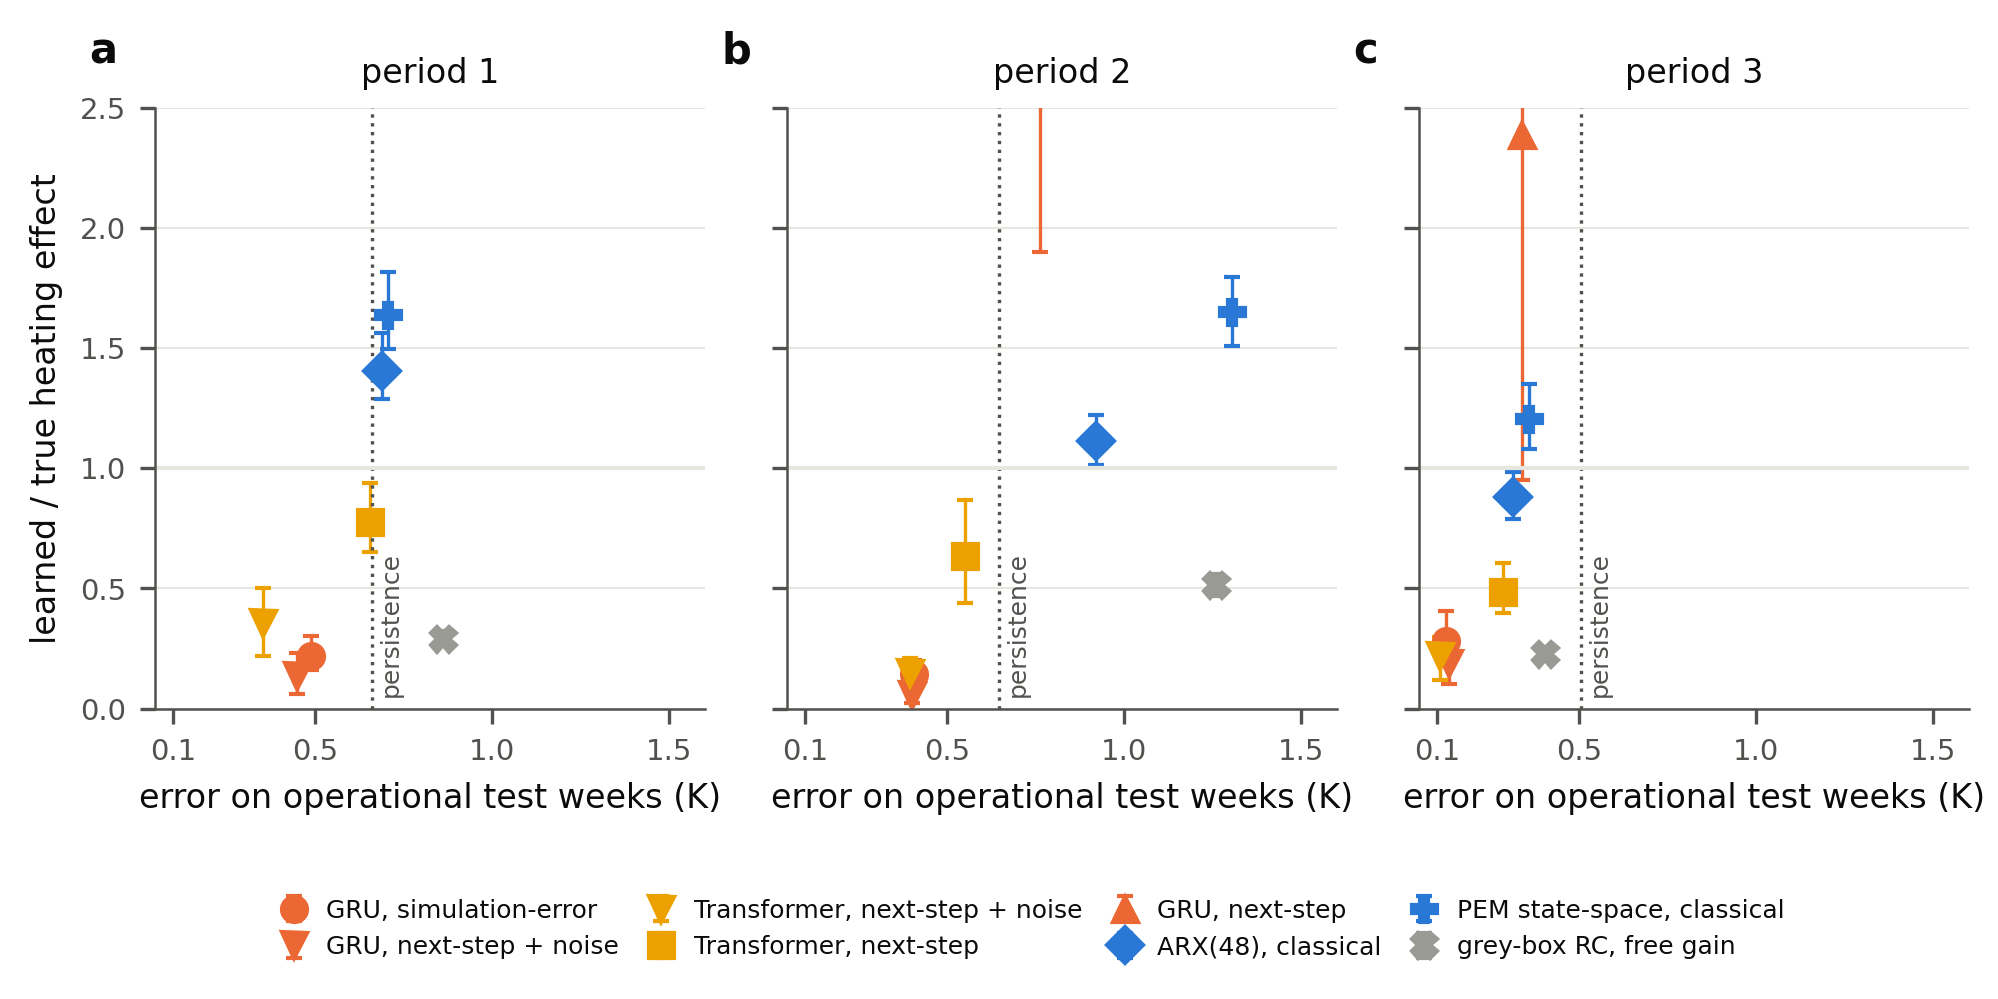
\includegraphics[width=\textwidth]{v1_figA_tradeoff.png}
\caption{\textbf{Operational accuracy against interventional fidelity, three heating-season periods.} Each point is a model family trained on the operational log of the BOPTEST heat-pump building: learned fraction of the true 24-h heating effect (step from seven operational start states 48~h apart; mean, 95\% hierarchical bootstrap interval over seeds and starts; five seeds for neural families) against the rollout error on the operational test weeks, the quantity practitioners validate on; dotted line, persistence. Simulation-error training and input-noise injection (orange and yellow triangles, circle) give the lowest operational errors and the lowest learned fractions; the classical direct methods (blue) over-estimate the effect in two periods; the clean next-step transformer (yellow squares) sits between.}
\end{figure}
\begin{figure}[p]\centering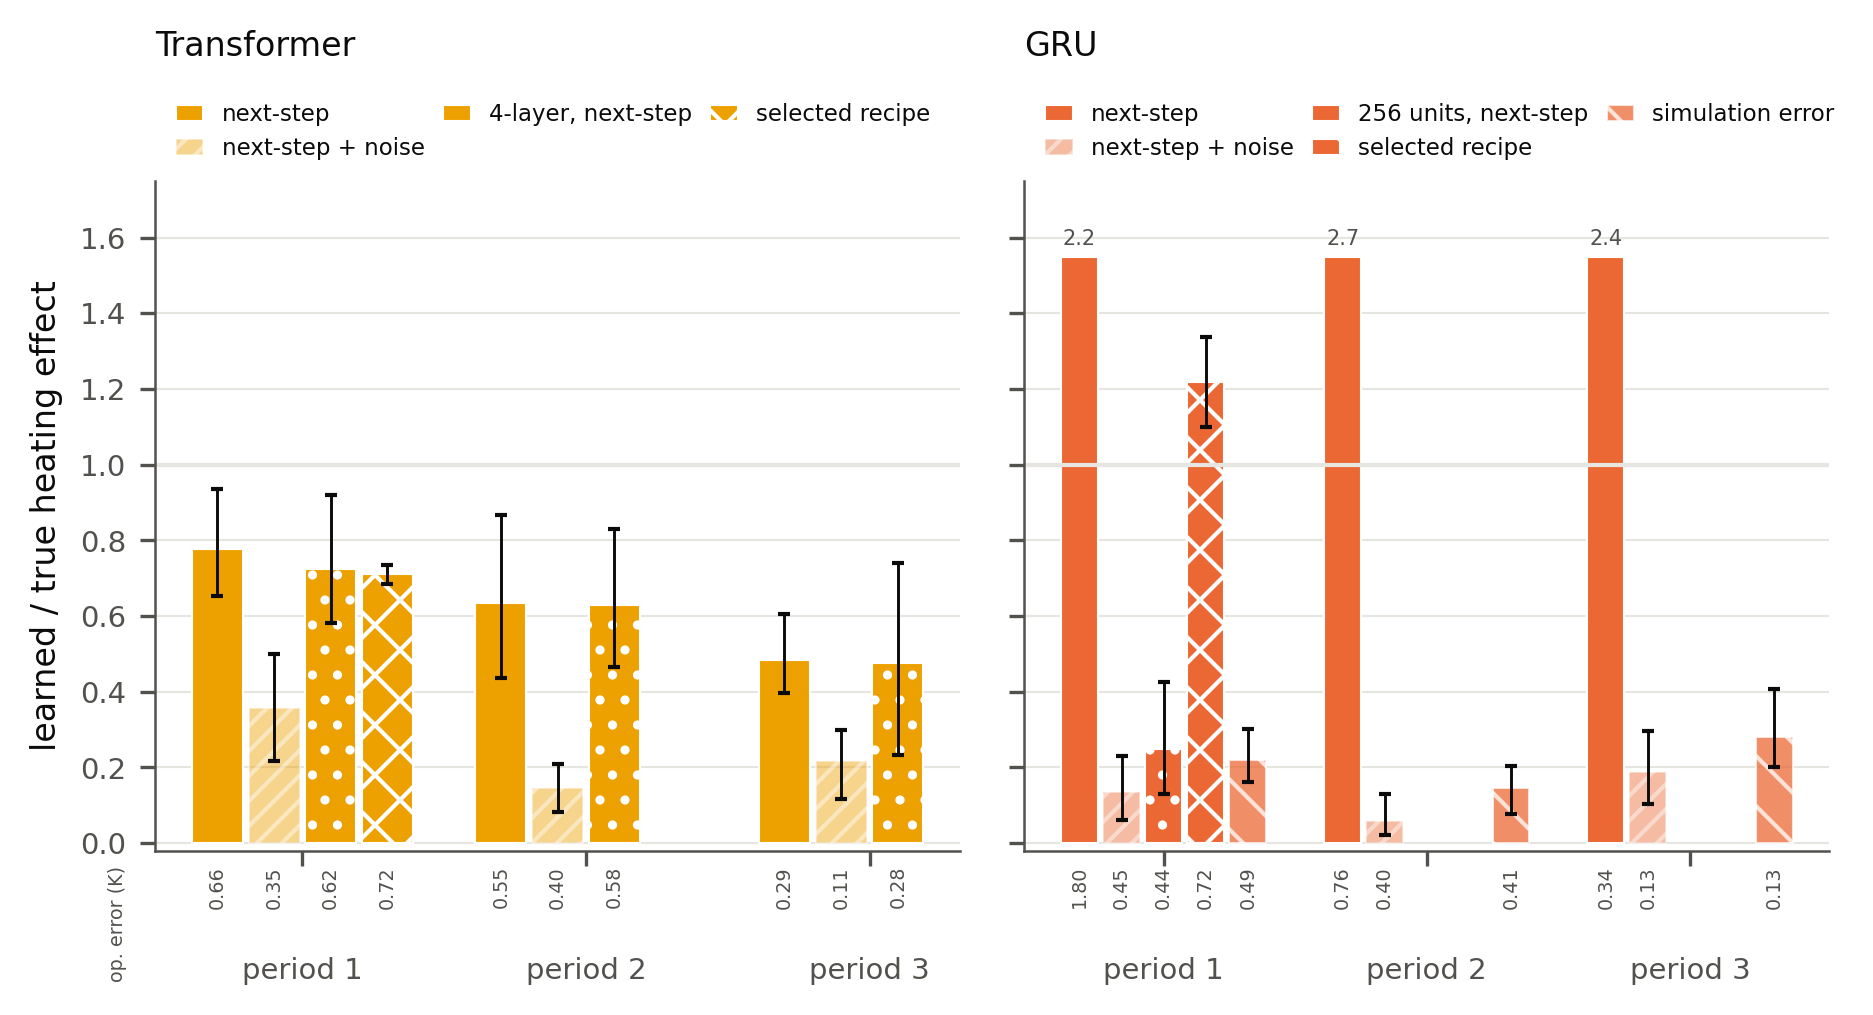
\includegraphics[width=0.8\textwidth]{v1_figD_ablation.png}
\caption{\textbf{Within one architecture, what buys operational accuracy buys the co-movement.} Learned 24-h fraction for the transformer and the GRU trained on the same operational log by next-step prediction with and without input-noise injection, at larger size (four layers; 256 units, period~1), with the recipe selected on designed data (period~1), and, for the GRU, by simulation error (five seeds, two to three for the large models; intervals as in Fig.~1; bars clipped at the axis are annotated with their values). The number under each bar is the twin's rollout error on the operational test weeks (K; persistence 0.66, 0.65, 0.51). The 48-unit clean GRU is not a working twin: on the in-range designed schedule its error is 3.5, 2.0 and 5.8~K against persistence 1.1, 1.7 and 1.4, and on operation it is worse than persistence in two periods; the 256-unit clean GRU reaches the simulation-error GRU's operational accuracy and its fraction. The selected-recipe bars show the range of two seeds, not a bootstrap interval.}
\end{figure}
\begin{figure}[p]\centering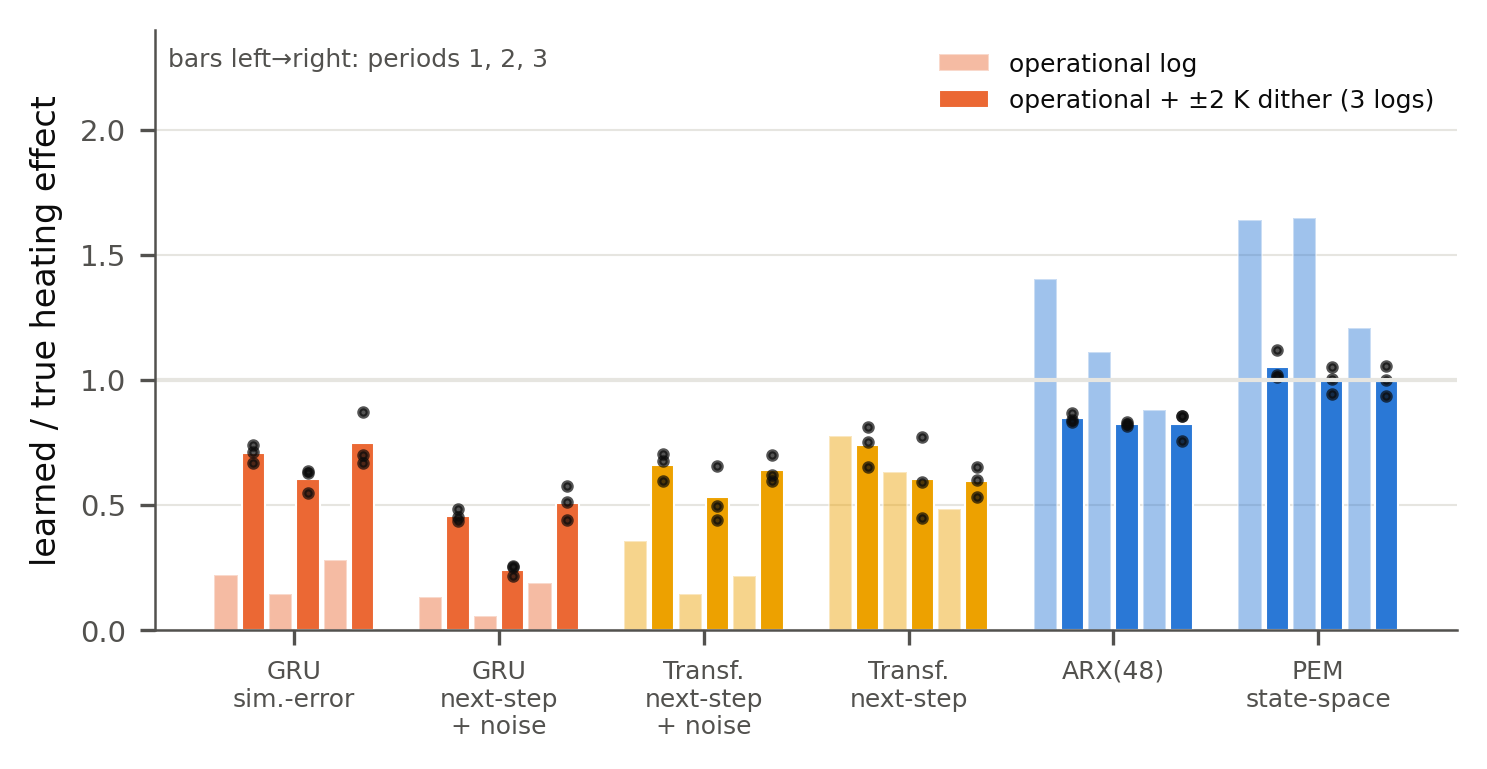
\includegraphics[width=0.9\textwidth]{v1_figB_dither.png}
\caption{\textbf{What a logged set-point dither buys.} Learned fraction for twins trained on the operational log (light) and on three logs with a $\pm2$-K random set-point offset (dark; dots, individual logs), by family and period.}
\end{figure}
\begin{figure}[p]\centering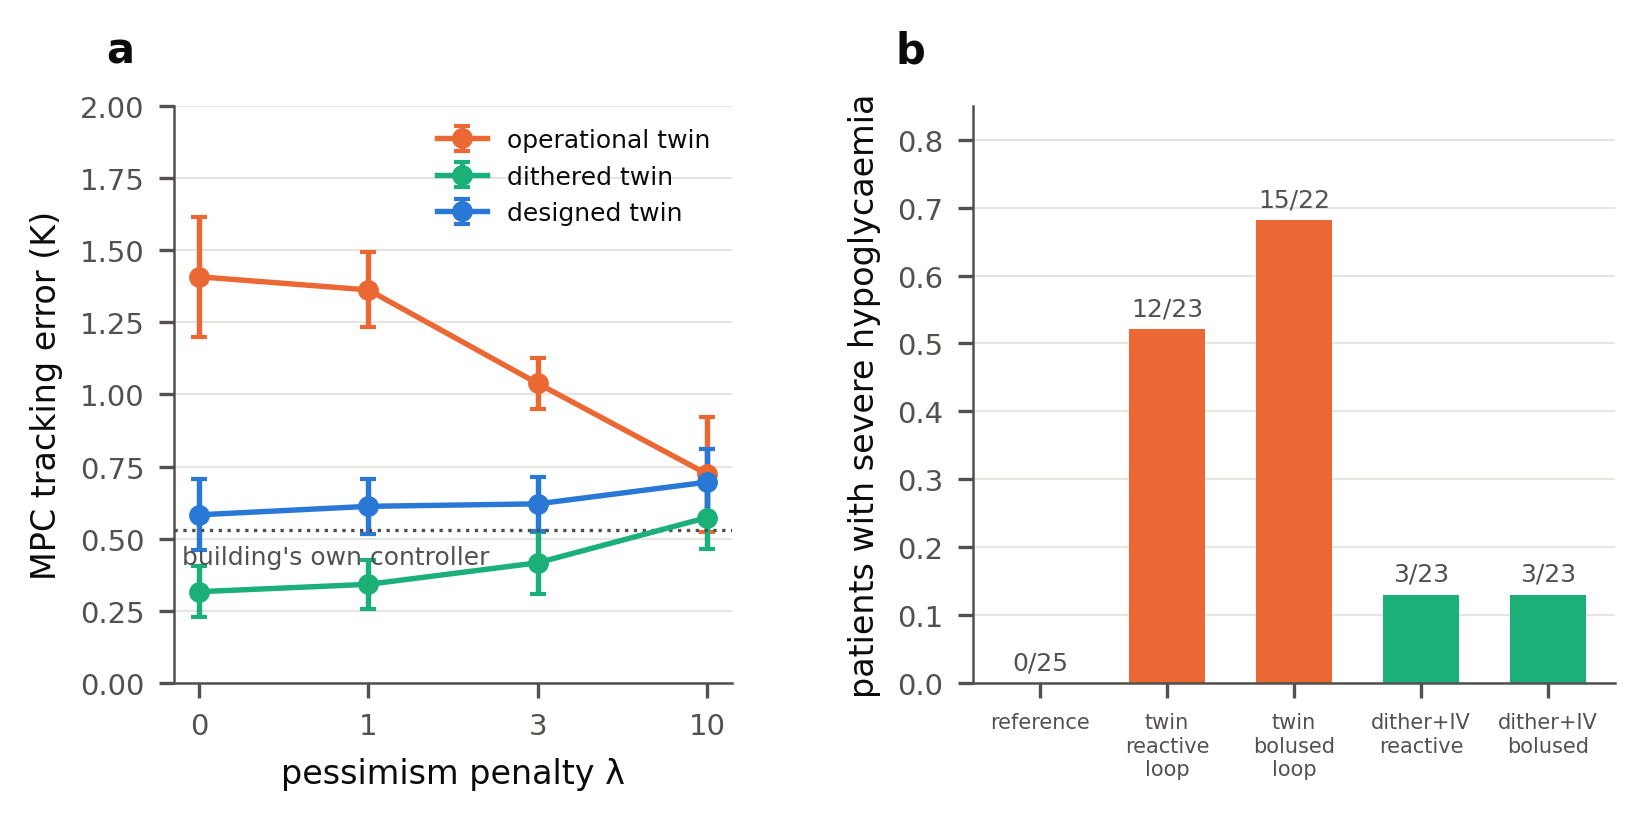
\includegraphics[width=0.9\textwidth]{v1_figC_decisions.png}
\caption{\textbf{Decisions.} \textbf{a}, Receding-horizon MPC through bootstrap ensembles of five twins on the building (twins trained on the period-1 logs of the first study version), for a set-point change that leaves the operating range (21.0 to 22.5~$^\circ$C), against the pessimism penalty on ensemble disagreement; dotted line, the embedded controller given the same target; five start times, mean $\pm$ s.d.; the in-range target (21.0 to 21.8~$^\circ$C) gives 0.66, 0.55, 0.30 and 0.59~K for the operational twin at $\lambda=0$ and 10, the dithered twin and the designed twin, against 0.47 for the controller (Supplementary Information). \textbf{b}, Diabetes simulator: fraction of 25 virtual patients driven below 54~mg/dL by a correction bolus computed from each twin's learned insulin effect, applied at a steady hyperglycaemia; the reference calculator uses the true effect at the same operating point.}
\end{figure}
\section*{Data availability}
All logs, step-response truths and model outputs are generated by the code below from the public BOPTEST test case (commit 0f8a467), the \texttt{simglucose} 0.2.11 virtual-patient library and a synthetic plant specified in Methods; the generated logs, step-response truths, per-model scores and result files that underlie every figure and table are deposited with the code at \url{https://github.com/DebojitBiswas/twins-co-movement} (Zenodo DOI to be added at acceptance).

\section*{Code availability}
The emulator interface, data-generation, training, evaluation and figure/table scripts (including the pre-registered protocol and the audit script that regenerates every number in the text) are available under the MIT licence at \url{https://github.com/DebojitBiswas/twins-co-movement}; the same scripts regenerate the Supplementary Tables from the result files.

\section*{Acknowledgements}
This work received no specific funding.

\section*{Author contributions}
D.B.\ conceived the study, designed and ran the experiments, analysed the data and wrote the paper.

\section*{Competing interests}
The author declares no competing interests.

\clearpage
\section*{Extended Data}
\paragraph{Extended Data Table 1 --- Pre-stated predictions and outcomes (corrected truth, seven 48-h-spaced starts).}
\emph{v1 building protocol} (written before any v1 model): V1, simulation-error GRU trained on operational logs learns $<50\%$ of the effect in all three periods: \textbf{met} (0.22, 0.14, 0.28); Chronos-2 could not be scored because it failed its capability control. V2, ARX($\ge12$)/PEM trained on operational logs within $\pm50\%$ in $\ge2$ of 3 periods with in-range error below persistence: \textbf{met for ARX} (1.40, 1.11, 0.88), \textbf{not met for PEM} (1.64, 1.65, 1.21). V3, clean next-step neural families between V1 and V2: \textbf{met for the transformer} (0.78, 0.63, 0.48), \textbf{not scorable for the 48-unit GRU} (unstable fits, rollouts worse than persistence; 0.25 at 256 units, 1.22 with the selected recipe). V4, $\pm2$-K dither raises the GRU's fraction in every period and seed: \textbf{met} (0.55--0.87 against 0.14--0.28, all nine logs). V5, pessimistic MPC not better than $\lambda=0$ by more than 20\%: \textbf{inconclusive}: out of range the paired per-start improvement is 0.68~K (s.d.\ 0.80, $n=5$, 4 of 5 starts better; $t=1.9$, two-sided $p=0.13$, 95\% CI $-0.31$ to $1.68$~K), in range 0.10~K (s.d.\ 0.17); the improvement comes with less heating and fewer out-of-range actions, consistent with retreat toward the behaviour policy, which the applied-input traces in Supplementary Note~8 show directly.
\emph{v0 synthetic kill criteria}: the first thesis (one-step high-order ARX fails under pure feedback) was \textbf{false} and led to the comparator design. \emph{v0 BOPTEST predictions}: P1 met on a post-hoc metric only; P3 half met; P5 (two-stage IV) not met and later found to be an estimator artefact. \emph{Theory programme}: T1 collapse met (synthetic); T2 conformal partially met (in-range coverage 40--81\%, not 0--5\%); T3 met; T4 ordinal; T5 downgraded; T6 modest; T7 monotone.

\paragraph{Extended Data Table 2 --- Register of changes made after seeing data.} v0: (1) BOPTEST reference signal corrected; (2) designed levels narrowed; (3) primary building metric changed to out-of-range do-RMSE (superseded by v1); (4) pancreas dither made additive; (5) one-step recipe changed (noise injection; now a labelled variant); (6) actuator what-if redefined; (7) certificate band chosen post hoc (certificate dropped); (8) a pre-run expectation about the commercial building's schedule was wrong; (9) GPU testbed withdrawn before its runs. v1: (10) in-range test levels tuned on the emulator before fitting; (11) levels scaled to the test period's operational heating level after period 3 under-heated; (12) dosing scenario revised twice (ramp overshoot; drip continuation); (13) pancreas exclusion threshold (50\% hypoglycaemia) set after v0; (14) planning target inside the range added after the referee round; (15) grey-box with free gain and Chronos-2 excluded by the pre-stated criterion (the sign-constrained simulation-error grey-box passes it in period~2 and is reported but not used as the comparator, because it over-estimates on designed data in the other two periods); (16) the emulator's Boolean override-activation inputs had been set as reals, which failed silently at some step-query starts (found by the second internal review round; fixed, truth regenerated, all models re-scored without retraining); (17) the step-query starts were 18--30~h apart instead of the stated 48~h (interleaving error; regenerated with seven starts 48~h apart); (18) the capability criterion's second clause (in-range error below persistence on designed data) had been dropped from Methods without registration; it is restored, and the designed-data twins' in-range errors are reported so that the reader can apply it (the simulation-error GRU fails the second clause in period~1 because the designed logs lie mostly outside the operating range, which is why the clause is informative about the log, not the twin). After the third internal review round: (19) the coherence band of the dither-log law test (3~h--2~days) was chosen after the fact; (20) a $+0.1$ step from the same start states and the per-horizon reporting were added because the $+0.3$ step's intervention arm leaves the training range for 67, 73 and 38\% of its first day; (21) the pancreas direct-method comparator was rerun on logs regenerated under the v1 protocol with a stable seed, since the v1 logs had been seeded with Python's per-process string hash and not saved; the earlier comparator used the ten-adult logs of the first study version; (22) the shuffled-day replay (the operational modulation sequence with its days permuted, replayed open-loop) was added after the fourth internal review round as the test that separates the controller's co-movement from the input spectrum; (23) the direct-method comparator was also fitted to the designed (open-loop) pancreas logs after the fourth round, to separate model-class failure from feedback bias in the reactive loop; (24) the dosing scenario was rerun with twin effects from the regenerated, saved pancreas logs.


\begin{figure}[h]\centering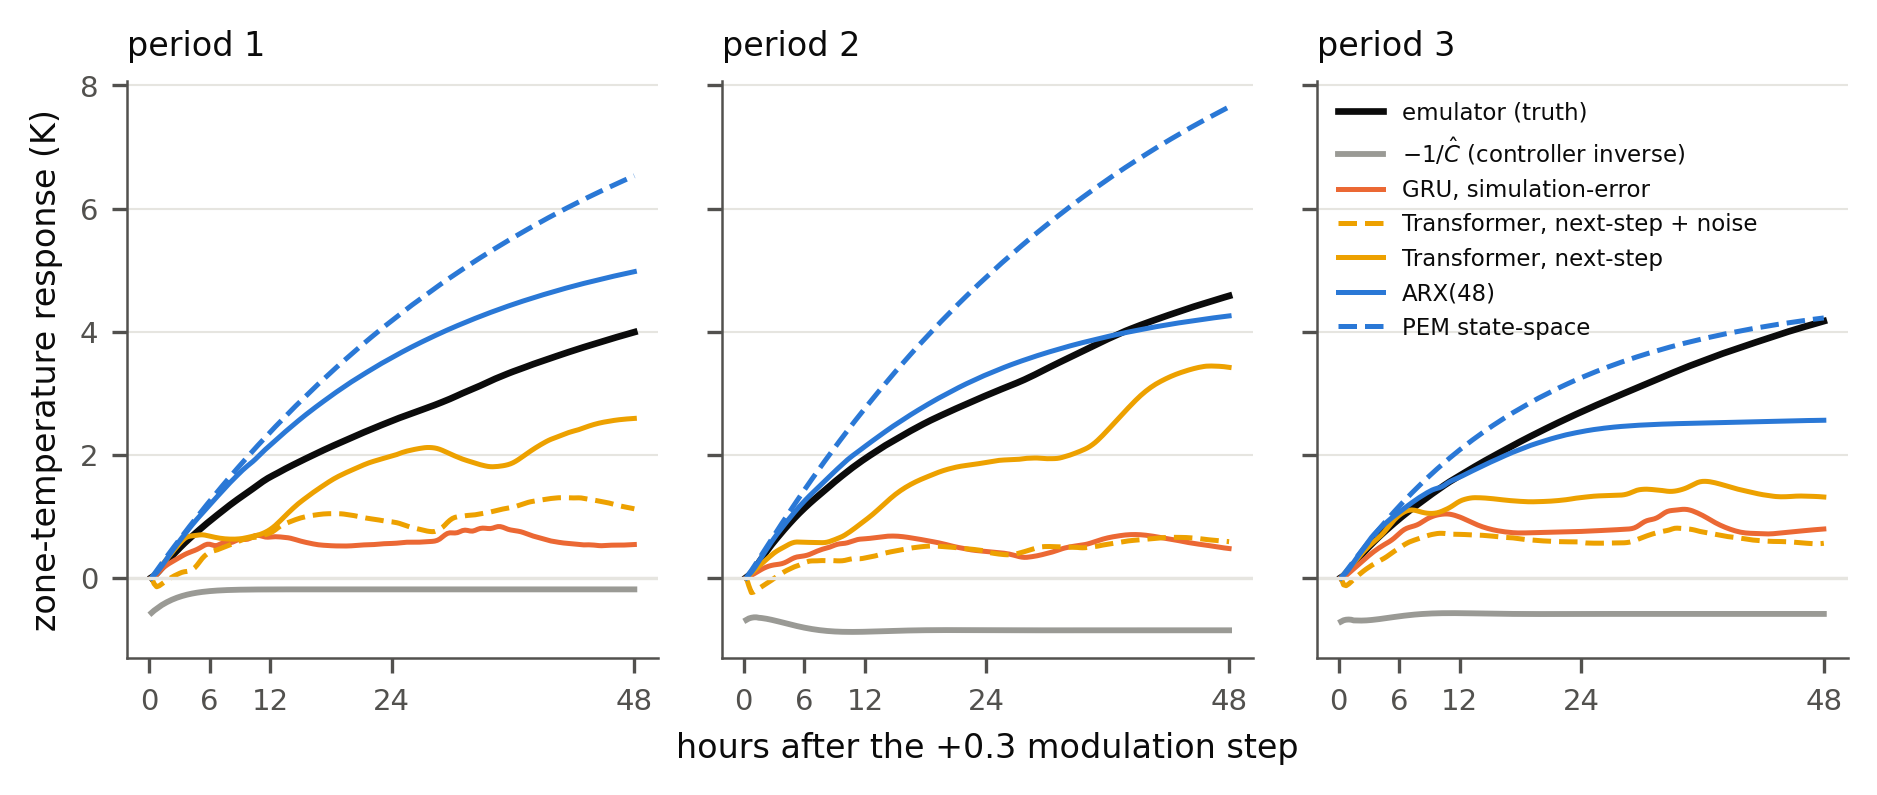
\includegraphics[width=\textwidth]{v1_figED11_invctrl.png}\caption*{\textbf{Extended Data Figure 1 --- Inverse-controller test, full trajectories.} For each period, the 48-h response to the $+0.3$ step of the emulator, of the fitted controller's negative inverse ($-1/\hat C$, ARX(6,6) fit of the embedded controller, $R^2>0.99$) and of the operational-data twins (mean over seeds); the inverse is largest in the first hours and decays toward zero under integral action, while the twins' responses are positive and, for the simulation-error and noise-injected families, a shrinking fraction of the truth with horizon.}\end{figure}
\bibliographystyle{plainnat}
\bibliography{refs}
\end{document}
